% ========================================================================== %
\section{Validation on simulations} \label{sec:simu}

In order to ensure that \panco\ is able to recover accurate pressure profile measurements, we test it on simulated inputs.
In this section, we detail this validation process, from the creation of the dataset to the results produces by \panco.
For reproducibility purposes, the datasets created and used for this analysis are made public with the software.

% -------------------------------------------------------------------------- %
\subsection{Sample selection}

The goal of the validation is to ensure that \panco\ is able to recover accurate pressure profiles from different types of data.
To that end, we seek to create realistic synthetic cluster maps from three instruments: the \textit{Planck} satellite, the South Pole Telescope (SPT), and the NIKA2 camera at the IRAM 30 m telescope.
The choice of these three instruments is motivated by their vastly different angular resolutions: the Compton$-y$ maps built from \textit{Planck} and SPT data have angular resolutions (expressed as the full width at half maximum, or FWHM) of 10 and 1.25 arcmin, respectively \citep{planck_collaboration_planck_2016, bleem_cmbksz_2022}, and the beam of the NIKA2 camera 150 GHz band -- used for tSZ mapping -- has an FWHM of 18 arcsec \citep{perotto_calibration_2020}.

We choose to create SZ maps for three clusters, labeled (C1, C2, C3), covering different regions of the mass-redshift plane:
\begin{alignat}{2}
    \nonumber {\rm C1}:\; & z=0.05,\ & M_{500} = 9 \times 10^{14} \ M_\odot ;\\
    \nonumber {\rm C2}:\; & z=0.5,\  & M_{500} = 5 \times 10^{14} \ M_\odot ;\\
              {\rm C3}:\; & z=1,\    & M_{500} = 3 \times 10^{14} \ M_\odot,
\end{alignat}
These mock clusters are shown as red stars in figure~\ref{fig:valid:sample}.
The top panel shows their positions in the mass-redshift plane, indicating that C1, C2 and C3 are realistic detections for the \textit{Planck}, SPT, and ACT tSZ surveys, respectively.
Tbe bottom panel of figure~\ref{fig:valid:sample} places the clusters in the angular diameter-redshift plane, showing that C1 can be resolved in \textit{Planck}, SPT, and NIKA2 tSZ maps, while C2 and C3 are too small to be resolved by \textit{Planck}.

\begin{figure}[tp]
    \centering
    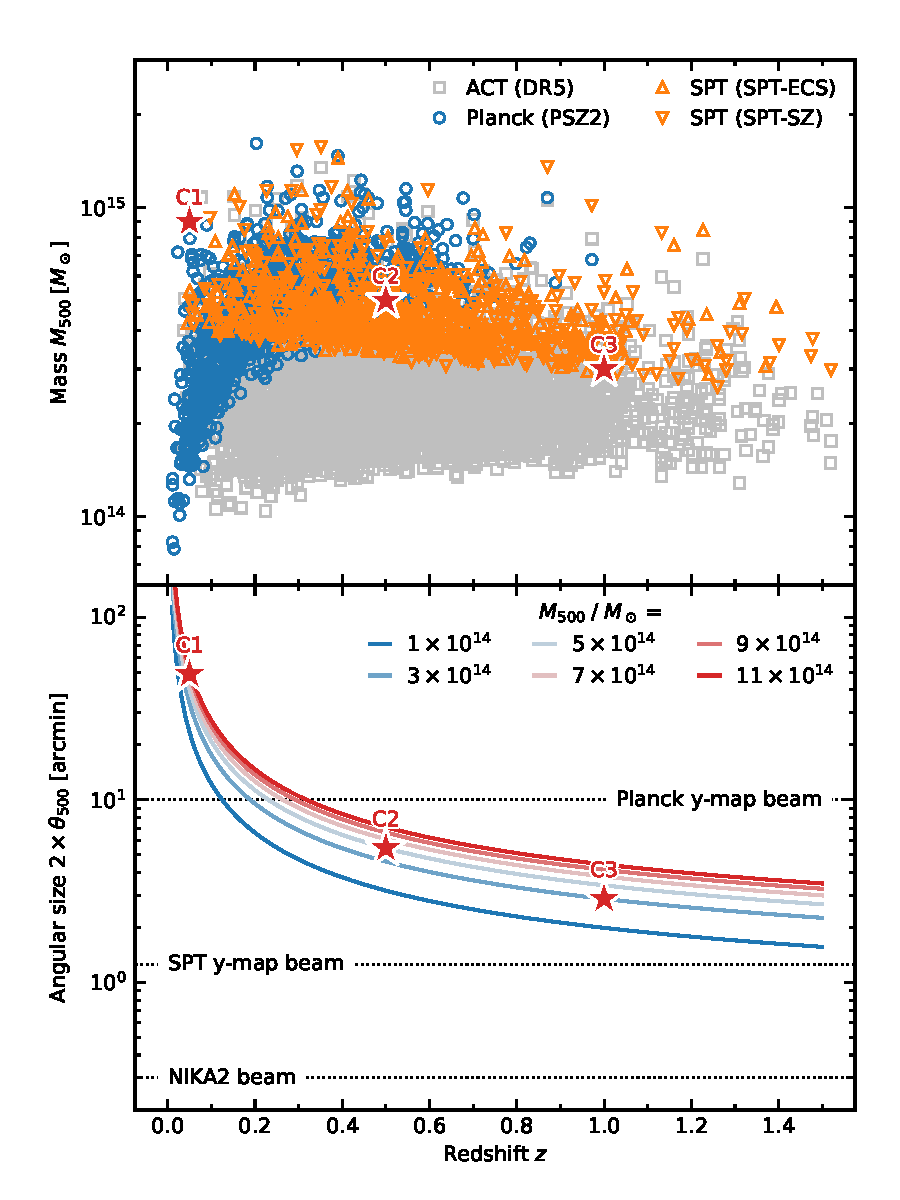
\includegraphics[width=\linewidth]{Figures/validation_sample.pdf}
    \caption{
        Validation cluster sample (red stars) in the mass-redshift plane (\textit{top panel}) and in the angular size-redshift plane (\textit{bottom panel}).
        For illustration, the top panel includes clusters detected in recent tSZ surveys: \textit{Planck} \citep{planck_collaboration_planck_2016-2}, ACT \citep{hilton_atacama_2021}, and SPT \citep{bleem_sptpol_2020,bleem_galaxy_2015}.
        Note that the redshift axis is truncated to $z<1.6$, therefore not showing all clusters in these samples.
        Colored lines in the bottom panel show the evolution of the angular $2\times\theta_{500}$ with redshift for clusters of different masses.
        The angular resolutions of the \textit{Planck} and SPT $y-$maps, as well as that of the NIKA2 camera at 150~GHz, are represented as dotted horizontal lines.
    }
    \label{fig:valid:sample}
\end{figure}

% -------------------------------------------------------------------------- %
\subsection{Data generation}

% -------------------------------------------------------------------------- %
\subsection{Pressure profile fitting}

% -------------------------------------------------------------------------- %
\subsection{Results}
